%!TEX root = ../report.tex


\chapter{Implementation}\label{ch:implementation}
As Trale is built with decentralization, flexibility, and micro-services in mind, the implementation had to be split into several parts.
This chapter will explain these parts, their functionality, and why they exist.

\section{Trale Libraries}\label{sec:libraries}
In the project, we tried to re-use as much code as possible.
Sine the client and server-side projects are both implemented in TypeScript, we moved shared logic between the projects into separate libraries.

Each library serves a different purpose in the Trale system, and is in-fact independent from each other.
Code contained in the libraries is more of a general approach to solve a certain problem.
Through delegation of specific tasks, the library stays flexible, while the concrete way of performing a task is implemented in the actual client application.
I.e. you may want to store data in an encrypted manner, so the library will take care of applying an encryption algorithm, while the consumer of the library provides the specific algorithm to be used.

However, due to some constraints of the TypeScript compiler, working with these libraries didn't work by creating a local connection to the package, but we had to upload them to npm and install them afterwards.
This lead to some issues in the development process, such as version mismatches between the server and client, where both had to use the newest version, but one was using an older version.

% TODO rename this chapter to make clear that the libraries are self-developed
% TODO @all add introduction to libraries
% -> why libraries?
% -> advantages?
% -> disadvantages?

\subsection{Transport}\label{subsec:transport}
One of the big questions during the project was: how can we get data (messages) from one client to another one and temporarily save data, which shall be sent to a user who is currently offline?
The former part of this question will be addressed by the Transport library, whilst the latter part is delegated to the library consumer, i.e. the node.js based chat server.

The Transport library, as the name suggests, is responsible for getting transporting data from one client to another (technically from a client to a server, and then to another client).
It only provides transport security for client-server connections!
The actual content of a message packet has to be properly encrypted by the client!

% TODO @joernneumeyer & @mauritsvanderzee
% TODO add link to npm
\paragraph{Establishing a Secure Client-Server Connection}
Although the content, and most meta data (e.g. time sent, sender name) of messages shall be encrypted by clients, some data has to be apparent to the server, in order to have the ability to forward the message to the proper recipient.

In order to establish a secure connection between a client and a server, both parties must be in possession of the following things:
\begin{itemize}
  \setlength\itemsep{-.5em}
  \item an \ac{ECDH} public and private key pair of curve P-384 \parencite{nist-digital-signature-standard}
  \item an RSA public and private key pair of length 4096-bit
\end{itemize}

The \ac{ECDH} keys are used to negotiate a common key, which can be used to encrypt data using AES.
The RSA keys are used to verify one's identity by means of digital signatures, so the other party knows that the handshake message hasn't been tampered with.

How the handshake works:
\vspace{-.75em}
\begin{enumerate}
  \setlength\itemsep{-.5em}
  \item Client connects to server.
  \item Client sends initial message: [\ac{ECDH}$_{pub}$ || RSA-SHA512$_{priv}$(\ac{ECDH}$_{pub}$)]
  \item Server calculates shared secret.
  \item Server sends reply: [\ac{ECDH}$_{pub}$ || RSA-SHA512$_{priv}$(\ac{ECDH}$_{pub}$)]
  \item Client verifies the server's \ac{ECDH} signature. If the verification fails, the handshake and connection will be terminated.
  \item Client calculates shared secret and sends their username.
  \item Server loads the proper client RSA public key and verifies their identity. If the verification fails, the handshake and connection will be terminated.
  \item If the handshake/connection haven't been terminated due to prior errors, a secure connection has been established, via which all future data will be sent.
\end{enumerate}

\subsection{Persistence}\label{subsec:persistence}
Security by means of encryption does not only apply to the transport step of data, but also to the way data is persisted.
However, it would be quite redundant to always manually specify the full path to a file one wants to operate on or the way data should be encrypted and decrypted.
Therefore, we created an abstraction to address these issues.

The persistence library offers a simple API to instantiate a so called \enquote{CryptoStorage}, which performs its operations on a given base directory with user-specifiable encryption algorithms.
Given a base directory, one can now easily perform operations relative to that directory without being bothered to know the actual full path.

The two most fundamental operation revolve around saving files in an encrypted manner and loading them from the local storage and retrieving the encrypted data in plain text again.
Additionally, another API for so called \enquote{TextRecordStorage}s is provided to stream the content of a file containing multiple sub-records.

\subsubsection{Streaming File Content - TextRecordStorage}
A \enquote{TextRecordStorage} is a helper, which stores multiple pieces of data in a text based format in one file.
This functionality could also be achieved using functions of the \enquote{CryptoStorage}, but the \enquote{TextRecordStorage} provides an important feature, which is missing in the \enquote{CryptoStorage}: streaming the content of a file instead of fully loading it in one go.
But why is this important?

One implication of a messenger, which is frequently used by a user, is, that over time a lot of messages will be accumulated in chat logs one has with varying chat partners.
These chat logs may become so large that they won't fit into a client's memory (RAM) at once.
Therefore the need to load message on an on-demand basis.

To achieve this on-demand loading, the \enquote{TextRecordStorage} loads the specified file in chunks (meaning smaller parts).
Next, each chunk will be checked, if it contains a full record.
If that's not the case, the next chunk will be loaded and concatenated with the previous one.
This process is repeated until the next record has been fully loaded.
As soon as this happens, the new record will be returned.

One important remark: all of the described (record) loading will only take place if a new record is requested.
If no are requested, no data will be loaded and the machines memory will not be utilized unnecessarily.
% TODO @joernneumeyer & @mauritsvanderzee
% TODO add link to npm

\subsection{Utilities}\label{subsec:utilities}
The utilities library contains various functionality which is of general use and not as specific as logic contained in prior libraries.
It basically serves as a collection of shared code, which is used in all backend services as well as the frontend client.
This functionality includes common helpers for security, express.js, and common data types;
% TODO @joernneumeyer & @mauritsvanderzee
% TODO add link to npm


\section{Frontend}\label{sec:frontend}

\subsection{Services}\label{subsec:services}

% TODO rework introduction section
The following part of the dossier will describe the different services which have been developed during the time of the project.
This will include a description of each service, followed by an REST API specification.

\subsubsection{API Service}\label{subsubsec:api-service}

The API service is a rather small service located in the desktop client.
The service is responsible for managing the global state of all relevant API information in the desktop application.
In the current state of development this includes the following information

\begin{itemize}\setlength\itemsep{-0.5em}
    \item hostname - the hostname of the server (e.g.\ trale.org)
    \item port - the default port on which the service is listening for incoming connections (default: 8086)
    \item the remote endpoint - a constructed string for building a connection to the server (e.g.\ http://trale.org:8086)
    \item trale port - the default port on which the service is listening for encrypted messages (default: 8087)
\end{itemize}

Further, the service provides several helper methods for retrieving and updating the remote endpoint as well as several
getters and setters for all above mentioned attributes.

\subsubsection{Auth Service}\label{subsubsec:auth-service}
The auth service is responsible for managing authentication related tasks such as login, logout, registration and
minor helper functions (e.g.\ forgot password).

\paragraph{Login function}
The login takes a username and a password as parameters and executes a post request to the remote endpoint specified in
the \textbf{\hyperref[subsubsec:api-service]{API service}}.
On a successful login a token will be provided for future authentication, otherwise an error stating 'Invalid
credentials - Status code 400' will be returned.

% TODO @joernneumeyer maybe add register / logout etc. here as well? refactor code? not in auth service yet

Due to the mentioned responsibilities, this service is only injected in authentication related components.

\subsubsection{Contact Service}\label{subsubsec:contact-service}

The contact service is responsible for managing all contact related tasks and corresponding state management.
It owns a contact array holding all contacts for the currently logged-in user.
On application startup the contact service will load all contacts from drive by utilizing the
\textbf{\hyperref[subsubsec:crypto-storage-service]{Crypto Storage Service}}.

Besides providing a loading wrapper for retrieving encrypted contacts from the drive it also manages actions such as
adding contacts, updating contacts or fetching the latest message of all contacts to display those in the contact list.

Lastly, the contact service provides a function to load the actual chat of a specific contact with the currently
logged-in user.

% TODO @joernneumeyer any additional remarks / information to be added?

\subsubsection{Debug Service?}
% TODO @joernneumeyer & @mauritsvanderzee
% @joernneumeyer shall we include debug service?

\subsubsection{Crypto Storage Service}
% TODO @joernneumeyer & @mauritsvanderzee

\subsubsection{Key Registry Service}
% TODO @joernneumeyer & @mauritsvanderzee

\subsubsection{Titp Service}
% TODO @joernneumeyer & @mauritsvanderzee

\subsubsection{Util Service}
% TODO @mauritsvanderzee

\subsection{Components}\label{subsec:components}


\section{Backend}\label{sec:backend}

\subsection{Database Connections}\label{subsec:database-connections}

For the project we used two database management systems, MongoDB and MySQL, depending on the requirements of the backend
services.

\subsubsection{MongoDB}
MongoDB is a non-relational, document based database management system.
This brings a few advantages ad disadvantages, depending on the use case.
MongoDB is best when you want the flexibility of schema.
You can easily use replica sets with MongoDB and can take advantage of scalability.
Expansion plans are flexible and can be easily achieved by adding more machines and RAM to the system.
It also includes document validations and integrated systems.

A big disadvantage of MongoDB is that over time the data size will increase drastically over time.
Compared to other DBMS systems the speed is comparatively low.

\paragraph{Why and where was MongoDB used?}
Mongo DB was used for the messages.
This is because the messages are non-relational data in the case of SocialStuff.
The disadvantage of low speed once the data amount increases is neglectable in the case of SocialStuff, as the data will
only be stored temporarily on the server.
The data amount is therefore not that high.
Of course local machines will still store the messages on a longer period, however as only the messages with chat
partners are stored the amount of data is still comparatively low.

Due to the high scalability of MongoDB it is excellent for SocialStuff, as the entire system is based on users adding
more servers to the system to increase the security of the system.

\subsubsection{MySQL}
MySQL is a relational database management system, this also features advantages and disadvantages.
For starters MySQL provides a high performance and runs on almost every system which is important for SocialStuff as
users will be able to setup the servers themselves.
Using MySQL will make this process simpler for them.
MySQL also provides a high security, because the database administrator can grant appropriate permissions to
applications that access stored procedures in the database without giving any permissions on the underlying database
tables.
A disadvantage of MySQL is that it becomes slower the more data is stored on it due to a high memory usage.

\paragraph{Why and where was MySQL used?}
MySQL was used for all the relational data, like the data used in the identity service (user data) and reporting
service.
This was done as this data is not mere transactional data (like the messages) but data that is meant to stay.
Furthermore, the high scalability will proof useful once the application will be used by more users and more than our
one test server is online.

\subsection{Services}\label{subsec:services2}

\subsubsection{Authentication Service}
% TODO @joernneumeyer

\subsubsection{File Service}
% TODO @all shall we just briefly mention that this might be a service for future features / development

\subsubsection{Identity Service}
\label{subsubsec:identitySer}
% TODO @joernneumeyer

\subsubsection{Settings Service}\label{subsubsec:settingsSer}

The Settings service provides an interface to the admin panel frontend and carries out the settings to the other
services.
This service was developed in parallel to the admin panel frontend. %TODO @maltecastner insert reference to component, once it has been added
First only the for the UI necessary functionality would be added, later on the actual functionality was added
(e.g.\ that users can actually be reported for the report reasons added in the settings).
As it can be seen from the use case diagram~\ref{fig:ucd} the settings service carries out a few tasks by itself whilst
forwarding certain other requests to the \hyperref[subsubsec:identitySer]{\textbf{identity service}} and the
\hyperref[subsubsec:reportingSer]{\textbf{reporting service}}.
The use cases as well as their descriptions are located in the
\hyperref[ch:software-requirements-specification-(srs)]{\textbf{\ac{srs}}}

\begin{figure}[!ht]
    \centering
    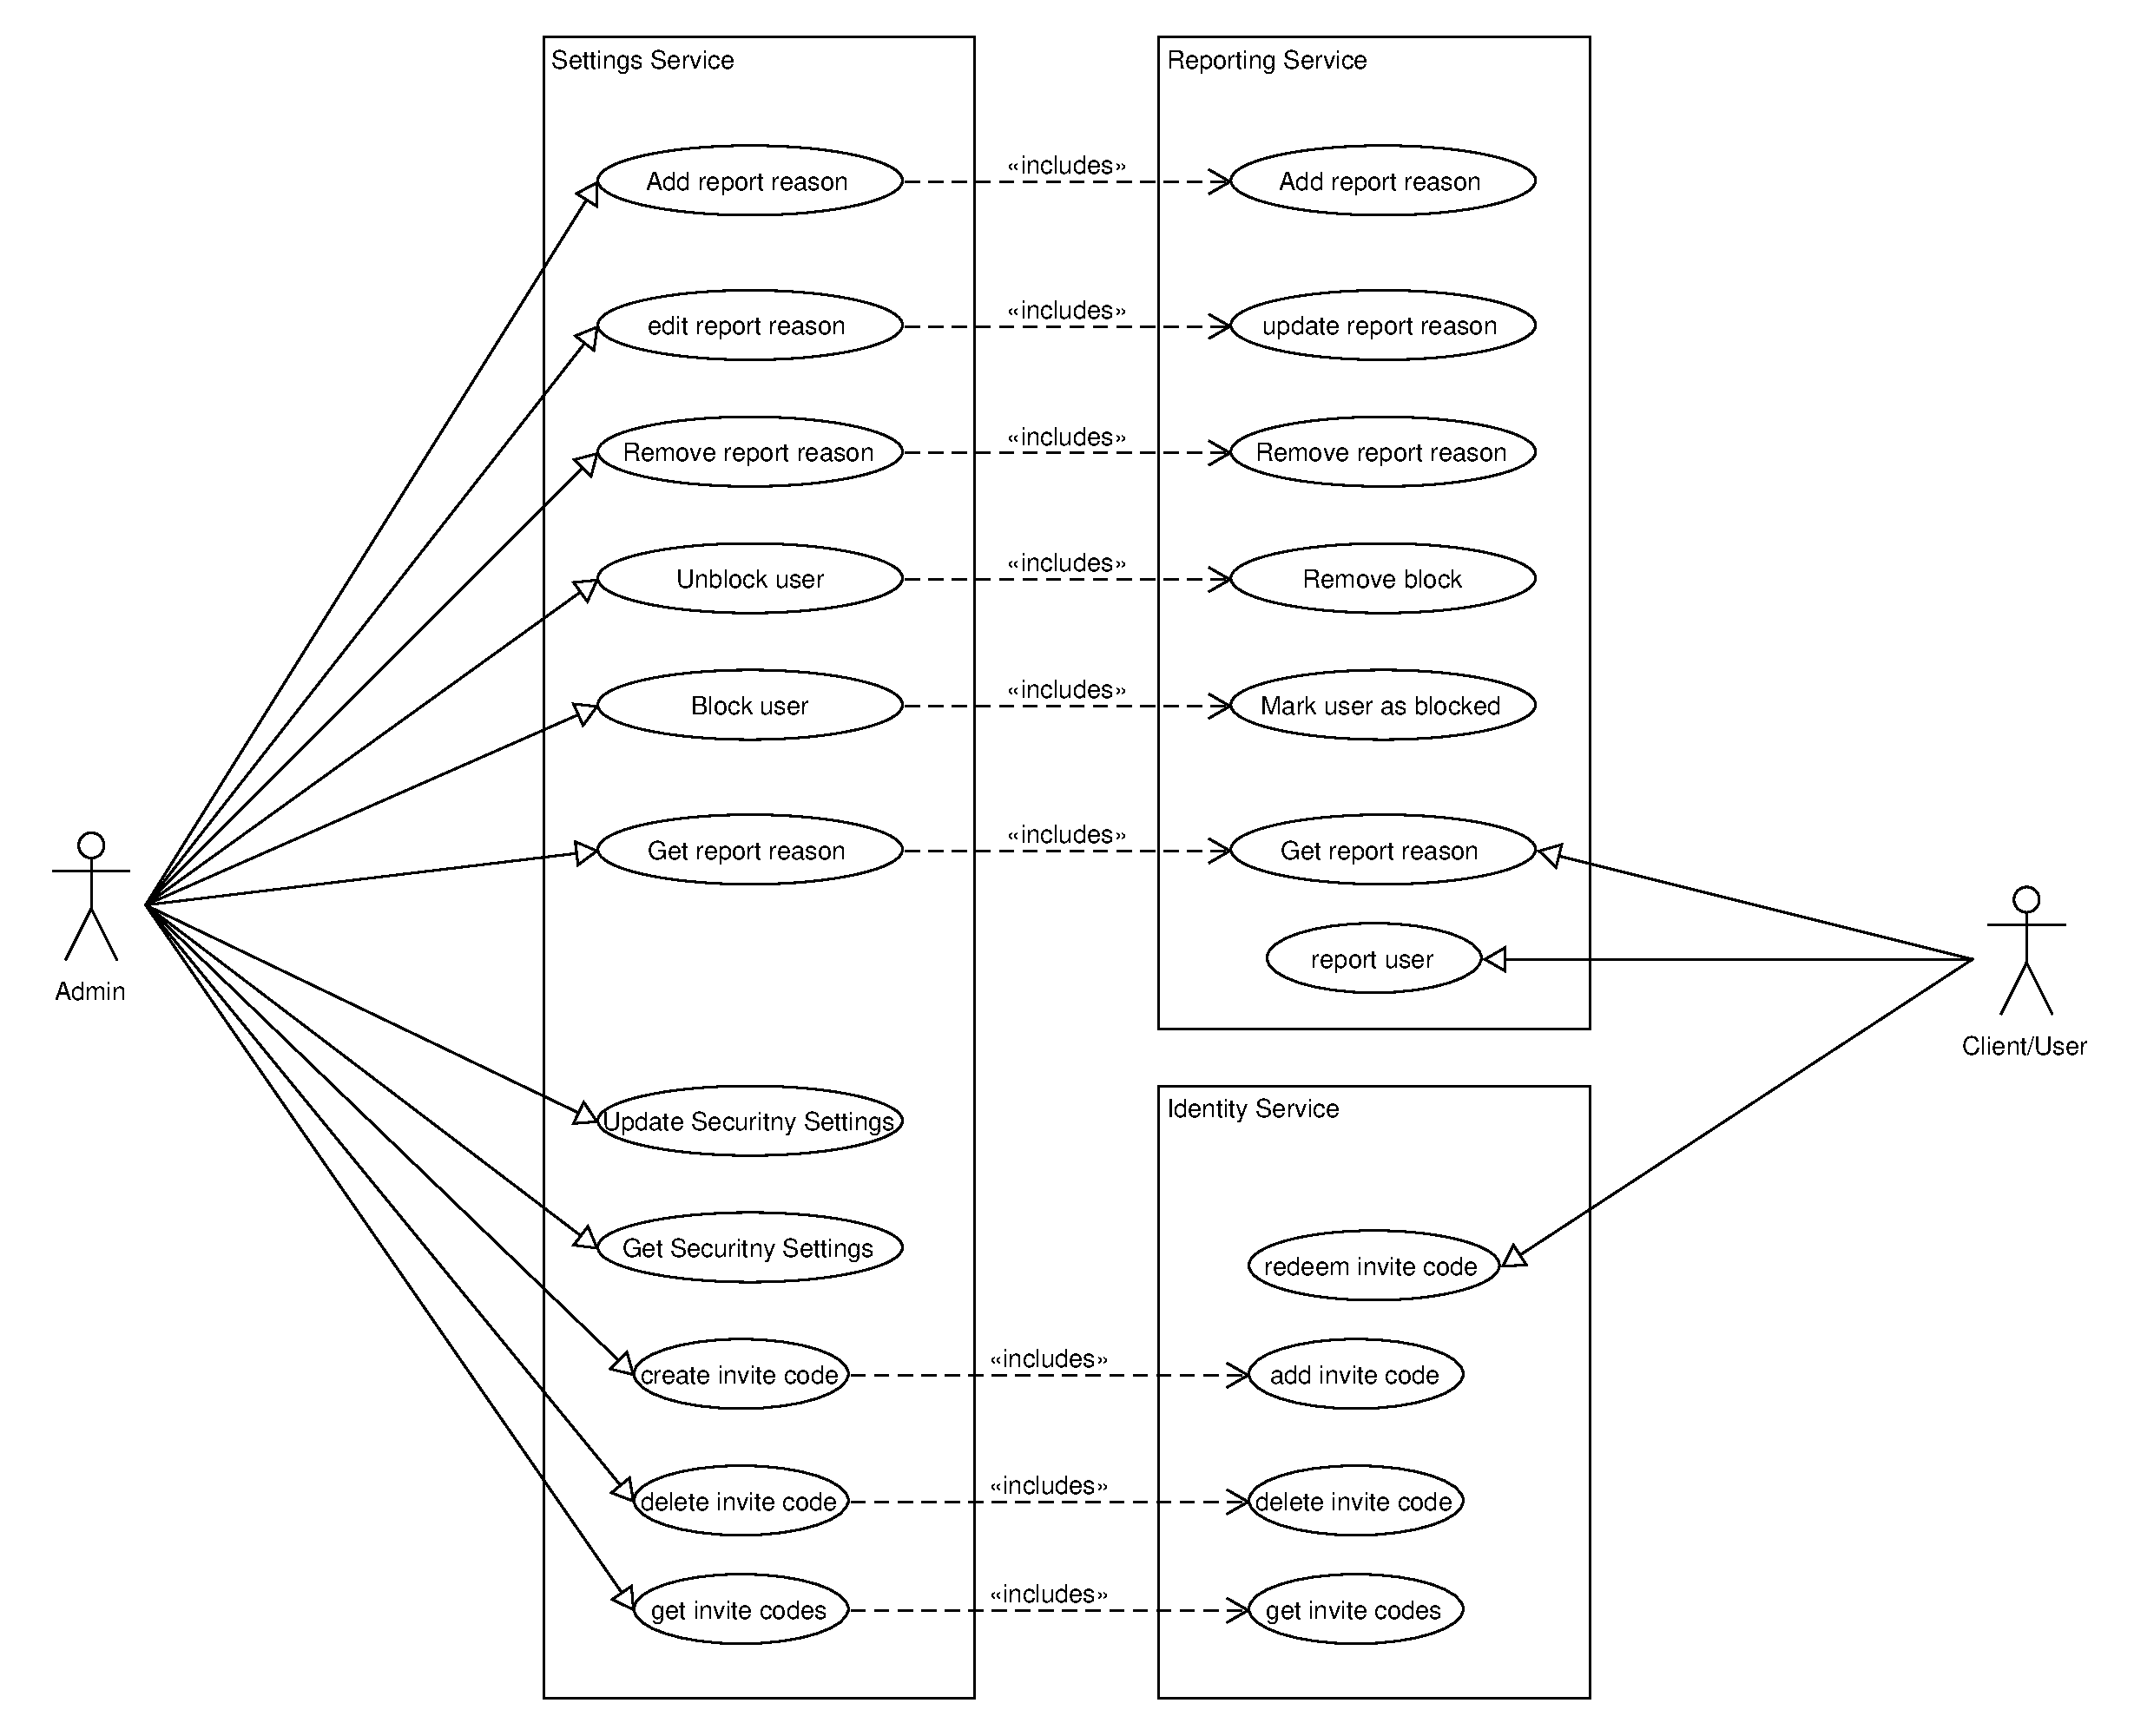
\includegraphics[width=1.0\textwidth]{./images/UseCaseDiagramAdminPanel}
    \caption{Use case diagram of the admin panel showing responsibility of each AP service}
    \label{fig:ucd}
\end{figure}

\paragraph{Rest interface}

The settings service provides the following rest endpoints:

\begin{lstlisting}[label={lst:lstlisting}]
GET: /settings/report-reason
\end{lstlisting}

Returns all report reasons as a JSON array.

\begin{lstlisting}[label={lst:lstlisting2}]
POST: /settings/report-reason
body:
{
"reason": "some reason",
"max_report_violations": 5
}
\end{lstlisting}

Adds a new report reason.

\begin{lstlisting}[label={lst:lstlisting3}]
PUT: /settings/report-reason
body:
{
"id": 123,
"reason": "some reason",
"max_report_violations": 5
}
\end{lstlisting}

Edits an existing report reason.

\begin{lstlisting}[label={lst:lstlisting4}]
DELETE: /settings/report-reason
headers:
- "id": 123
\end{lstlisting}

Deletes a report reason with an id that is provided as a header.

\begin{lstlisting}[label={lst:lstlisting5}]
GET: /settings/security
\end{lstlisting}

Returns the current security settings.

\begin{lstlisting}[label={lst:lstlisting6}]
PUT: /settings/security
body:
{
    "two_factor_auth": {
    "on" : true,
    "phone": false,
    "email": true
},
    "confirmed_emails_only": true,
    "individual_pwd_req": {
    "on": true,
    "upper_case": true,
    "number": true,
    "special_char": true,
    "reg_ex": false,
    "reg_ex_string": "[]"
},
    "inv_only": {
        "on": false,
        "inv_only_by_adm": false
    }
}
\end{lstlisting}

Edits the security settings.
The new settings are provided in body.

\paragraph{Example add report reason}

\begin{figure}[!ht]
    \centering
    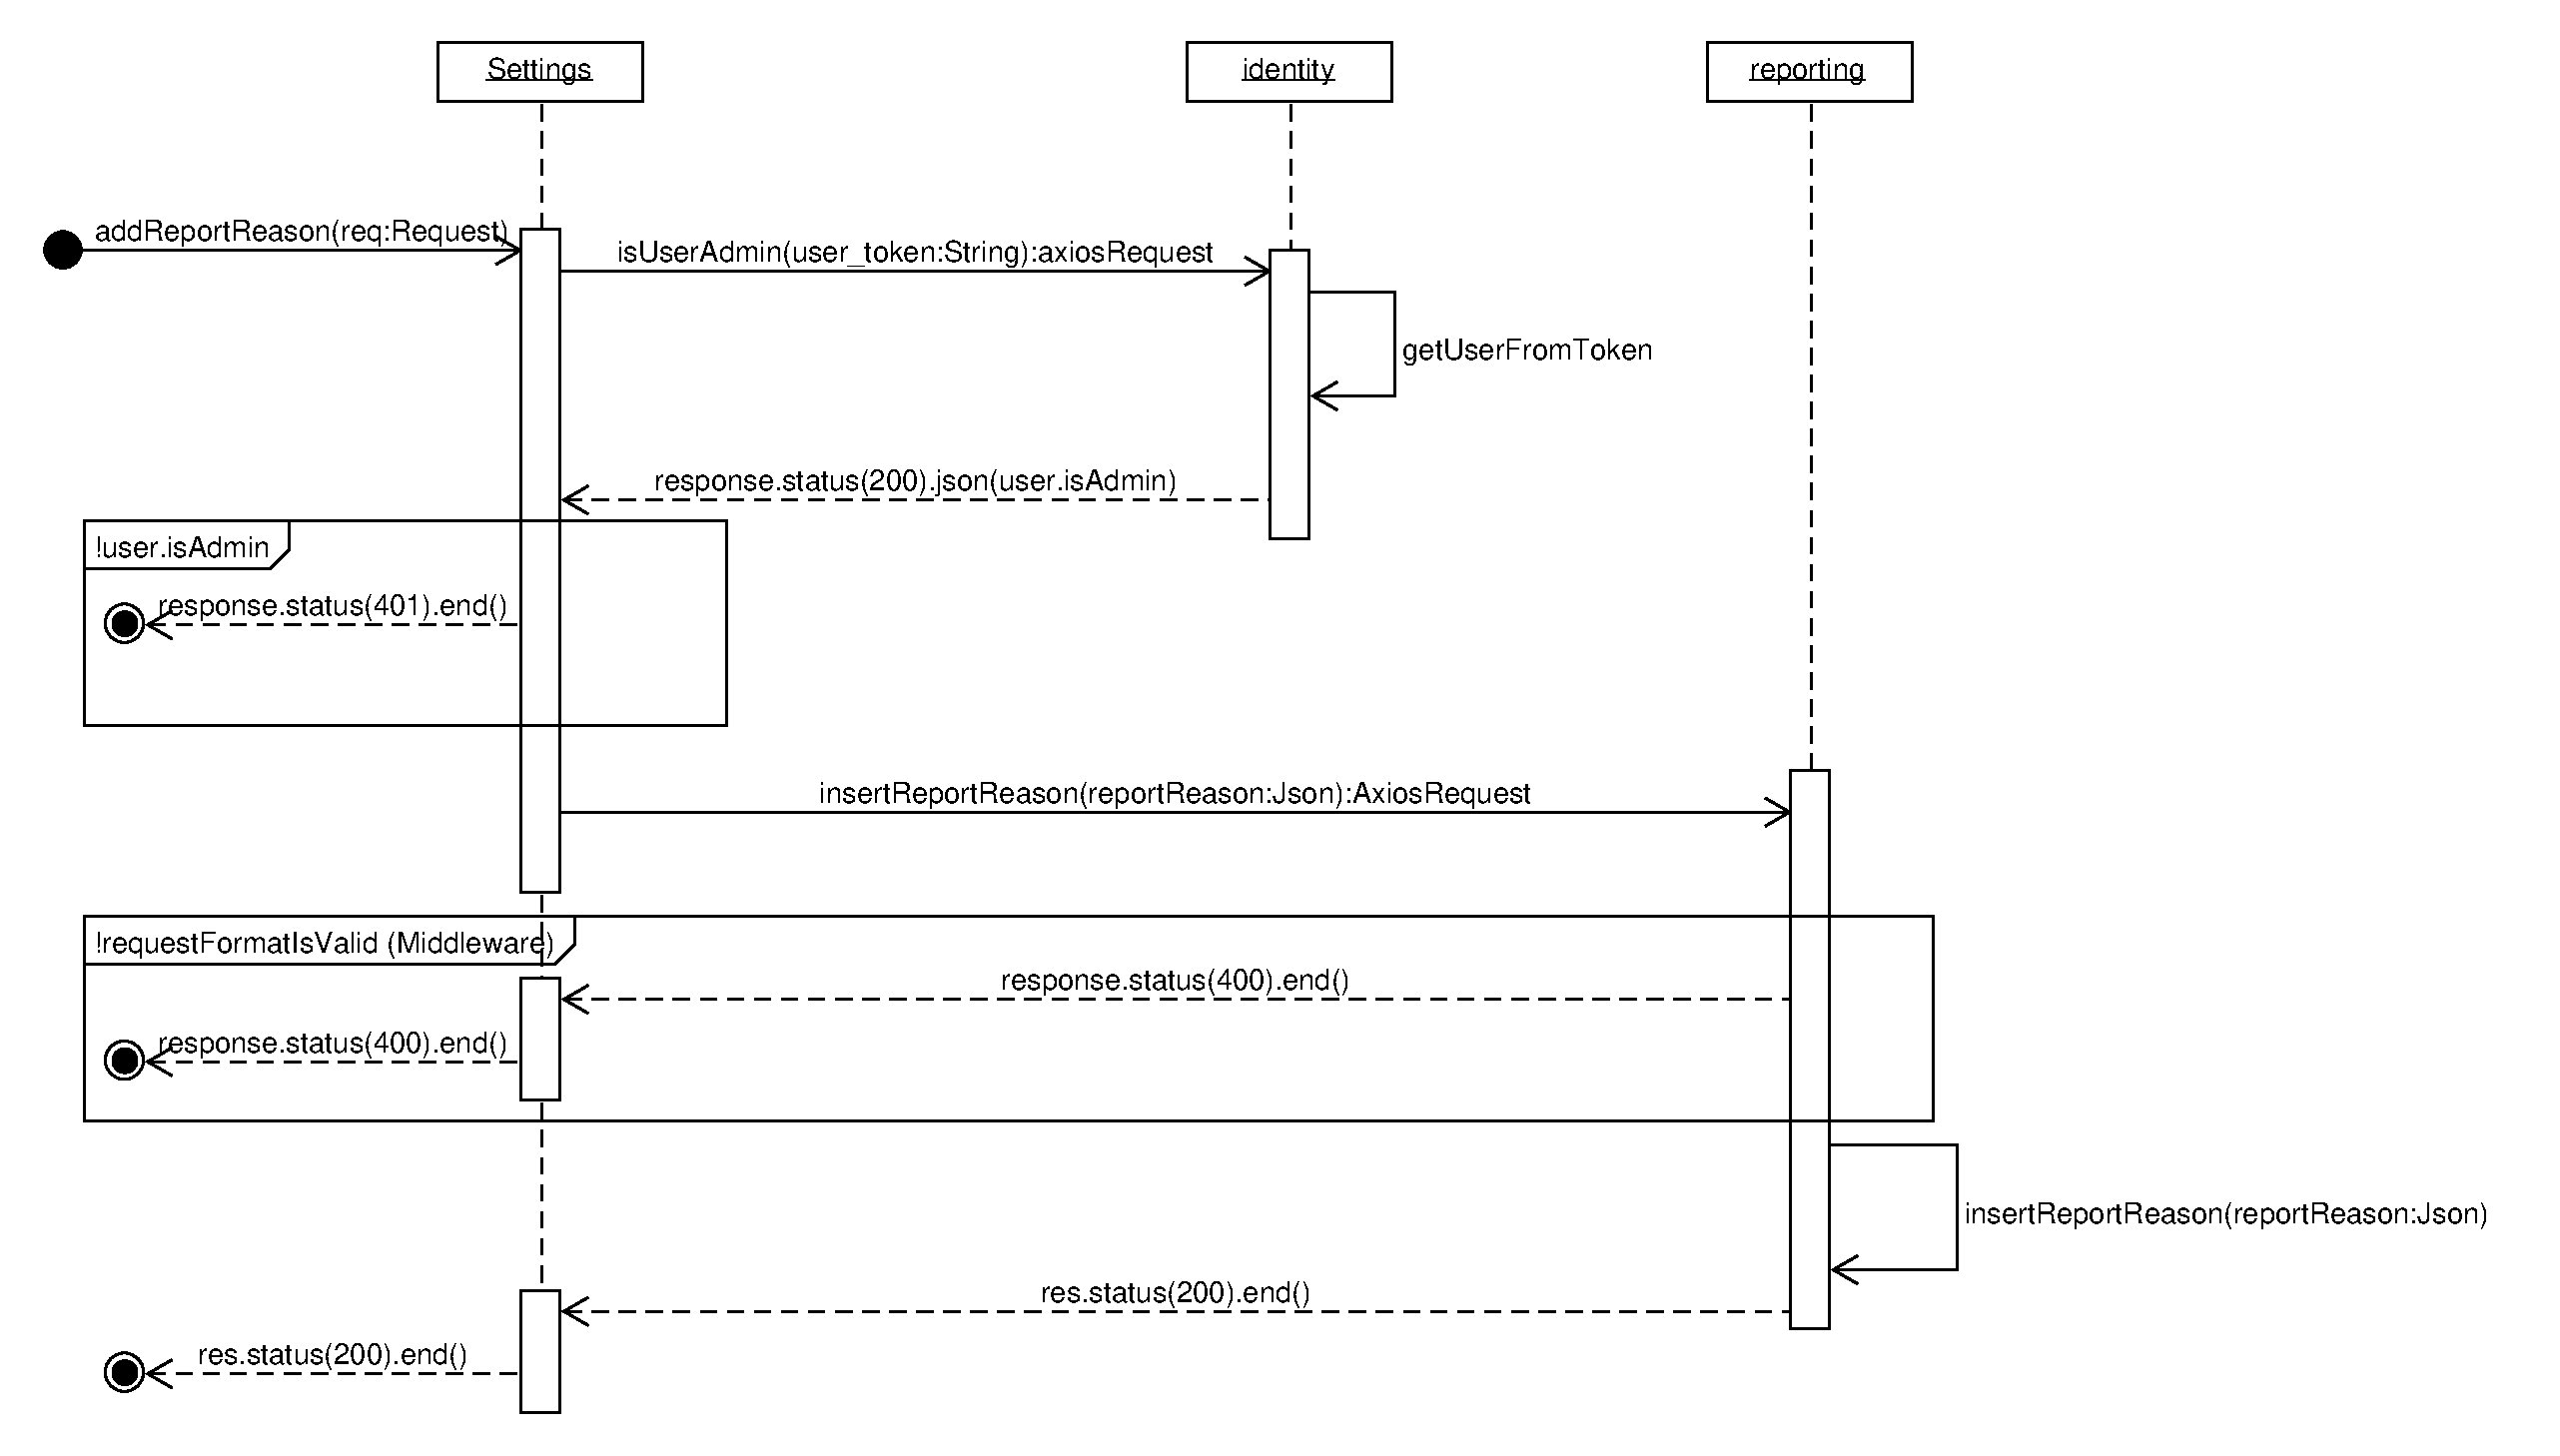
\includegraphics[width=1.0\textwidth]{./images/SequenceDiagram_AddReportReason}
    \caption{Use case diagram of the admin panel showing responsibility of each AP service}
    \label{fig:addReportReason}
\end{figure}

The sequence diagram~\ref{fig:addReportReason} shows an example of the communication of the settings service with the
aforementioned services.
The event is triggered by a request from the client.
Firstly the settings service will be verifying the identity of the sender by checking at the identity service, if the
user who sent out the request is in fact an administrator.
Then the request will e forwarded to the reporting service.
Here it will be checked if the request format is valid.
Should this not be the case, the reporting service will return an error (status 400).
Otherwise, the reason will be added in the reporting database, which will then be returned to the settings service,
who will then let the client know by response that the insertion was a success.
This way each service has a clearly defined task.

\subsubsection{Reporting Service}\label{subsubsec:reportingSer}

The reporting service handles the reporting system.
This includes administrative tasks like managing for which reasons users can be reported, as well as the reporting
system itself (reporting users and banning them).
The administrative tasks, like adding new report reasons, manually blocking and unblocking users, can be done via the
\hyperref[subsubsec:settingsSer]{\textbf{settings service}}.
This service was added in the later stages of the project.

First the entire reporting was handled via the \hyperref[subsubsec:settingsSer]{\textbf{settings service}}, however it
was decided that the reporting itself should possess its own service. % TODO @tobiasjansen --> why? explanation missing
Therefore, it was necessary to outsource the report related functionality from the
\hyperref[subsubsec:settingsSer]{\textbf{settings service}} to the
\hyperref[subsubsec:reportingSer]{\textbf{reporting service}}.

\paragraph{Rest Interface}
\begin{lstlisting}[label={lst:lstlisting7}]
POST: /report-reasons
body:
{
    "reason": "some reason",
    "max_report_violations": 5
}
\end{lstlisting}

Adds a new report reason returning the ID of the added report reason.

\begin{lstlisting}[label={lst:lstlisting8}]
PUT: /report-reasons
body:
{
    "id": 12
    "reason": "some reason",
    "max_report_violations": 5
}
\end{lstlisting}

Edits a report reason by the \enquote{ID} key and returns the edited reason.

\begin{lstlisting}[label={lst:lstlisting9}]
GET: /report-reasons
\end{lstlisting}

Returns all existing report reasons as JSON array

\begin{lstlisting}[label={lst:lstlisting10}]
DELETE: /report-reasons
headers
    - id: 12
\end{lstlisting}

Deletes a report reason by ID which is provided in the header of the request.
Returns the ID of the deleted request in its body.

\begin{lstlisting}[label={lst:lstlisting11}]
Headers:
    - user_token
Body:
{
    "username": "userHashOfUserBeingReported",
    "reason_id": 123
}
\end{lstlisting}

Reports a user based of the report reason, and the users' username hash.
A user can only be reported by the same user for the same reason after 15 minutes to prevent spamming.
Otherwise, the report will be processed by the backend, and the user will be set to \enquote{blocked} in case one
exceeds the maximum report violation counter.

